\documentclass[10pt]{article}

\usepackage[a4paper, left=2cm, right=2cm]{geometry} % A4 paper size and thin margins

\usepackage{xcolor} % Required for specifying custom colours
\definecolor{grey}{rgb}{0.9,0.9,0.9} % Colour of the box surrounding the title

\usepackage{graphicx}
\usepackage[colorlinks=true, allcolors=black]{hyperref}
\usepackage{amsmath}
\usepackage{indentfirst}
\setlength{\parindent}{2em}

\usepackage[utf8]{inputenc} % Required for inputting international characters
\usepackage[T1]{fontenc} % Output font encoding for international characters
\usepackage[sfdefault]{ClearSans} % Use the Clear Sans font (sans serif)
%\usepackage{XCharter} % Use the XCharter font (serif)
\usepackage{float}
\usepackage{listings}
\newcommand{\tabincell}[2]{\begin{tabular}{@{}#1@{}}#2\end{tabular}} 	

\begin{document}
%----------------------------------------------------------------------------------------
%	TITLE PAGE
%----------------------------------------------------------------------------------------

\begin{titlepage} % Suppresses displaying the page number on the title page and the subsequent page counts as page 1
	
	%------------------------------------------------
	%	Grey title box
	%------------------------------------------------
	
	\colorbox{grey}{
		\parbox[t]{1.1\textwidth}{ % Outer full width box
			\parbox[t]{1.02\textwidth}{ % Inner box for inner right text margin
				\raggedleft % Right align the text
				\fontsize{34pt}{40pt}\selectfont % Title font size, the first argument is the font size and the second is the line spacing, adjust depending on title length
				\vspace{0.7cm} % Space between the start of the title and the top of the grey box
				
				< Journey Assistant >\\
                Delivery List\\
                Version 1.0\\
				
				\vspace{0.7cm} % Space between the end of the title and the bottom of the grey box
			}
		}
	}
	
	\vfill % Space between the title box and author information
	
	%------------------------------------------------
	%	Author name and information
	%------------------------------------------------
	
	\parbox[t]{1\textwidth}{ % Box to inset this section slightly
		\raggedleft % Right align the text
		\large % Increase the font size
		{\Large Group Member}\\[4pt] % Extra space after name
        Yiwen Song\\
        Zhihui Xie\\
        Weizhe Wang\\
        Huangfei Jiang\\
        Haoping Chen\\
		% Institution Name\\[4pt] % Extra space before URL
		% \texttt{LaTeXTemplates.com}\\
		
		\hfill\rule{0.2\linewidth}{1pt}% Horizontal line, first argument width, second thickness
    }
    
	
\end{titlepage}

\newpage

\begin{center}
    {\LARGE Modification History}
    
    \begin{tabular}{|c|c|c|c|} 
        \hline 
        Date&Version&Description&Author\\
        \hline  
        2019-06-18&1.0&Finish the first version.&Weizhe Wang\\
		\hline 
		& & & \\
		\hline
		& & & \\
		\hline
		& & & \\
		\hline
    \end{tabular}    
\end{center}

\newpage

\tableofcontents
\newpage

\section{Intruduction}
\subsection{Purpose}
This delivery list is to list what we need to delivery about the Journey Assitant software and give proper explanition. The list will show composition of all our document and software in our project. This document is written for users to check and accept the job of developers.

\subsection{Scope}
The document is written for our Journey Assistant software, and all content of accords with the software's features, subsystems, models, codes, etc.

\subsection{Definition}
The terms referred to in this document are defined in the project glossary document (Glossary.pdf).

\subsection{Bibliography}
\begin{itemize}
	\item[1.] <Object Oriented Software Engineering (Version 3)> (Tsinghua University Press)
	\item[2.] <Object Oriented Software Engineering Practice Guidelines> 
\end{itemize}

\subsection{Sketch}
This document includes document list and software list. Document list will list kinds of document and corresponding name. Software list will give every software module in the project and its filename as well as size. The two parts complement and contrast each other, will show our delivery together.

\section{Document List}
\subsection{Planning Stage}
Documents in planning stage are shown in Table \ref{Planning Stage}.
\begin{table}[htb]
	\centering 

	\begin{tabular}{c|c|c} 
		\hline 
		filename&file type&file size\\
		\hline  
Feasibility Analysis Report&pdf&130KB\\
\hline
Project Development Plan&pdf&133KB\\
\hline
Risk list&xlsx&10KB\\
\hline
\end{tabular}

\caption{Planning Stage}
\label{Planning Stage}
\end{table}

\subsection{Requirement Acquisition and Analysis Stage}
Documents in requirement acquisition and analysis stage are shown in Tabel \ref{Requirement Acquisition and Analysis Stage}
\begin{table}[htb]
	\centering

	\begin{tabular}{c|c|c} 
		\hline 
		filename&file type&file size\\
		\hline  
Glossary&pdf&24KB\\
\hline
Software Requirement Specification&pdf&516KB\\
\hline
\end{tabular} 
\caption{Requirement Acquisition and Analysis Stage}
\label{Requirement Acquisition and Analysis Stage}
\end{table}

\subsection{Design Stage}
Documents in design stage are shown in Table \ref{Design Stage}.
\begin{table}[htb]
	\centering

	\begin{tabular}{c|c|c} 
		\hline 
		filename&file type&file size\\
		\hline  
Software Architecture Document&pdf&2063KB\\
\hline
Software Design Model&pdf&1655KB\\
\hline
\end{tabular}
\caption{Design Stage}
\label{Design Stage}
\end{table}

\subsection{Test, Conclusion And Delivery Stage}
Documents in test, conclusion and delivery stage are shown in Table \ref{Test, Conclusion And Delivery Stage}.
\begin{table}[htb]
	\centering

	\begin{tabular}{c|c|c} 
		\hline 
		filename&file type&file size\\
		\hline  
Delivery List&pdf&263KB\\
\hline
Software Testing Plan&pdf&50KB\\
\hline
Software Testing Summary Report&pdf&42KB\\
\hline
Software Project Summary Reort&pdf&165KB\\
\hline
Software Acceptance Report&pdf&40KB\\
\hline
User Manual&pdf&7658KB\\
\hline
\end{tabular}
\caption{Test, Conclusion And Delivery Stage}
\label{Test, Conclusion And Delivery Stage}
\end{table}

\section{Software List}
\subsection{Android Client}
The name of our android project is TravelingAgent, the size of whole file is 480MB, and the structure of project is as follows:

\begin{figure}[H]
	\centering
	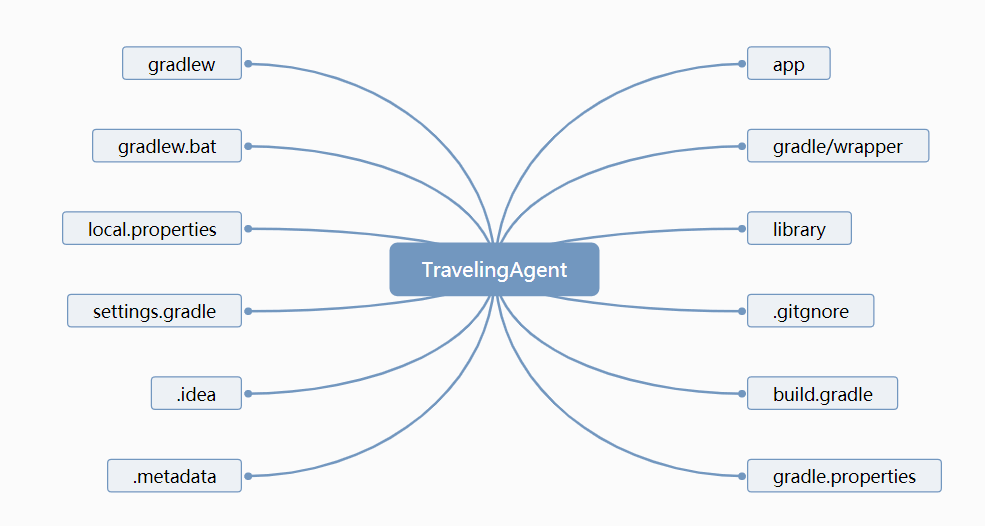
\includegraphics[width=14cm]{android.png}
	\caption{Android Client}
	\label{Android Client}
\end{figure}

\subsubsection{Java Source Code}
\begin{figure}[H]
	\centering
	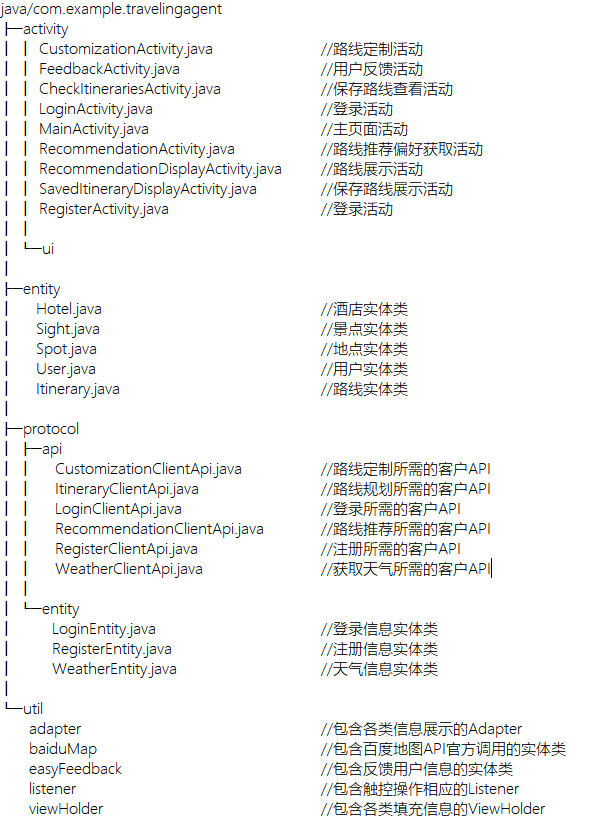
\includegraphics[width=7cm]{java.png}
	\caption{Java Source Code}
	\label{Java Source Code}
\end{figure}

\subsubsection{Resource File}
\begin{figure}[H]
	\centering
	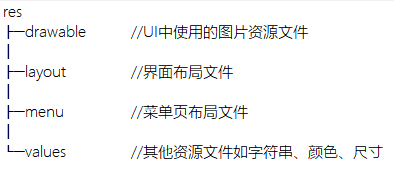
\includegraphics[width=7cm]{res.png}
	\caption{Resource File}
	\label{Resource File}
\end{figure}

\subsection{Server}
During constructing the server, the IDE we used is NetBeans IDE 8.2, and the server we userd is apache-tomcat-9.0.20, The name of file is jsf-helloworld with a size of 20.4MB, the file structure of project is as follow:

\begin{figure}[H]
	\centering
	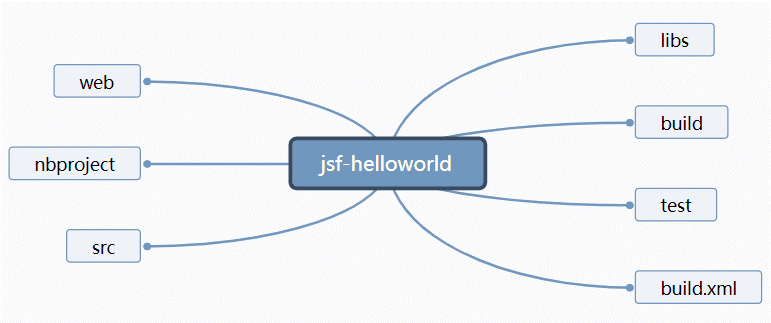
\includegraphics[width=14cm]{server.png}
	\caption{Server}
	\label{Server}
\end{figure}

Corresponding Java codes are in src, total size is 112KB, all the files are listed as follow:

\begin{figure}[H]
	\centering
	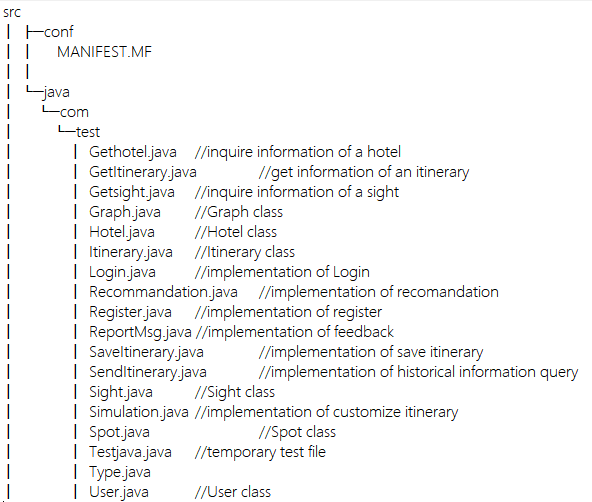
\includegraphics[width=7cm]{server_tree.png}
	\caption{Java Source Code}
\end{figure}

The libraries we used are listed as follow:

\begin{figure}[H]
	\centering
	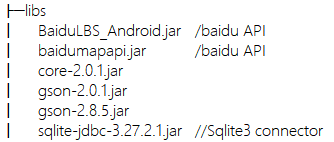
\includegraphics[width=7cm]{lib.png}
	\caption{Libraries}
\end{figure}

\subsection{Database}
\subsubsection{Overview}
Our software uses Sqlite3 to store the information. Our database file name is SEDB.db , with a size of 368KB. Since the database will be updated every month, it would be even larger in the future.

\subsubsection{Details}
Here is the property of tables in our database.

\begin{table}[htb]
	\centering

	\begin{tabular}{c|c|c|c|c|c}
		\hline
		Number&Field&Description&Type&Allow Null&Primary Key\\
		\hline
		1&ID&ID of users&int&N&Y\\
		\hline
		2&username&name of users&text&N&N\\
		\hline
		3&userpwd&password of users&text&N&N\\
		\hline
		4&mail&e-mail of users&text&N&N\\
		\hline
   \end{tabular}
	
	\caption{User}
\end{table}

\newpage

\begin{table}[htb]
	\centering

	\begin{tabular}{c|c|c|c|c|c}
		\hline
		Number&Field&Description&Type&Allow Null&Primary Key\\
		\hline
		1&sight\_id&ID of each sight&int&N&Y\\
		\hline
		2&name&name of each sight&text&N&N\\
		\hline
		3&popularity&popularity of each sight&double&N&N\\
		
		\hline
		4&price&price of each sight&double&N&N\\
		\hline
		5&total&total score of each sight&double&N&N\\
		\hline
		6&environment&environment of each sight&double&N&N\\
		\hline
		7&service&service score of each sight&double&N&N\\
		\hline
		8&latitude&latitude of each sight&double&N&N\\
		\hline
		9&longitude&longitude of each sight&double&N&N\\
		\hline
		10&city\_id&the id of city where sight lies&int&N&N\\
		\hline
		11&description&description of sight&text&N&N\\
		\hline
   	\end{tabular}
	\caption{Sight}
\end{table}

\begin{table}[htb]
	\centering

	\begin{tabular}{c|c|c|c|c|c}
		\hline
		Number&Field&Description&Type&Allow Null&Primary Key\\
		\hline
		1&hotelt\_id&ID of each hotel&int&N&Y\\
		\hline
		2&name&name of each hotel&text&N&N\\
		\hline
		3&popularity&popularity of eachhotel&double&N&N\\
		\hline
		4&price&price of each hotel&double&N&N\\
		\hline
		5&total&total score of each hotel&double&N&N\\
		\hline
		6&latitude&latitude of each hotel&double&N&N\\
		\hline
		7&longitude&longitude of each hotel&double&N&N\\
		\hline
		8&city\_id&the id of city where hotel lies&int&N&N\\
		\hline
		9&description&description of hotel&text&N&N\\
		\hline
   \end{tabular}
	\caption{Hotel}
\end{table}

\begin{table}[htb]
	\centering

	\begin{tabular}{c|c|c|c|c|c}
		\hline
		Number&Field&Description&Type&Allow Null&Primary Key\\
		\hline
		1&ItineraryID&ID of each itinerary&int&N&Y\\
		\hline
		2&city\_id&the id of city that user chooses&int&N&N\\
		\hline
		3&user\_id&ID of users&int&N&N\\
		\hline
		4&itinerary&the itinerary that user chooses&text&N&N\\
		\hline
   \end{tabular}
	\caption{User History}
\end{table}

\newpage

\begin{table}[htb]
	\centering

	\begin{tabular}{c|c|c|c|c|c}
		\hline
		Number&Field&Description&Type&Allow Null&Primary Key\\
		\hline
		1&msg\_id&ID of each message&int&N&Y\\
		\hline
		2&user\_id&ID of user that sends message&int&N&N\\
		\hline
		3&msg&content of message&text&N&N\\
		\hline
   \end{tabular}
	\caption{Feedback}
\end{table}
\end{document}
